% ---------------------------------------------------------------------------
% VT analysis report — LaTeX template
%
% Rendered by analysis.py with Jinja2. Values are inserted with VAR placeholders
% and logic with BLOCK statements. Edit the layout and wording freely; keep the
% placeholders. Figures are vector PDFs in report/figures/.
% ---------------------------------------------------------------------------
\documentclass[11pt,a4paper]{article}

% Computer Modern, LaTeX's default typeface (classic OT1 encoding, Type 1 fonts)
\usepackage[utf8]{inputenc}
\usepackage[a4paper,margin=2.4cm,top=2.3cm,bottom=2.6cm]{geometry}
\usepackage{microtype}
\usepackage{graphicx}
\usepackage{booktabs}
\usepackage{tabularx}
\usepackage{array}
\usepackage[table]{xcolor}
\usepackage{caption}
\usepackage{enumitem}
\usepackage{titlesec}
\usepackage{fancyhdr}
\usepackage{amsmath}
\usepackage{amssymb}
\usepackage{float}
\usepackage[round]{natbib}
\usepackage{needspace}
\usepackage[hidelinks]{hyperref}

\definecolor{ink}{HTML}{121211}
\definecolor{muted}{HTML}{6E6D68}
\definecolor{accent}{HTML}{1F5FAD}
\definecolor{rule}{HTML}{C9C8C0}

\graphicspath{{figures/}}
\setlength{\parindent}{0pt}
\setlength{\parskip}{0.55em}
\renewcommand{\arraystretch}{1.18}
\setlength{\aboverulesep}{0.25ex}
\setlength{\belowrulesep}{0.4ex}

\titleformat{\section}{\Large\bfseries\color{ink}}{\thesection}{0.7em}{}
\titleformat{\subsection}{\large\bfseries\color{ink}}{\thesubsection}{0.6em}{}
\titlespacing*{\section}{0pt}{1.6em}{0.6em}
\titlespacing*{\subsection}{0pt}{1.2em}{0.35em}
\newcommand{\keep}[1]{\Needspace{#1\baselineskip}}

\captionsetup{font=small,labelfont=bf,labelsep=period,justification=raggedright,singlelinecheck=false,skip=4pt}
\captionsetup[table]{position=top}

\renewcommand{\labelitemi}{$\bullet$}  % keeps every glyph in Type 1 Computer Modern
\newcommand{\note}[1]{{\footnotesize\color{muted}#1\par}}
\newcolumntype{R}{>{\raggedleft\arraybackslash}X}
\newcolumntype{L}{>{\raggedright\arraybackslash}X}

\pagestyle{fancy}
\fancyhf{}
\renewcommand{\headrulewidth}{0pt}
\fancyfoot[L]{\footnotesize\color{muted} Vanguard Total World Stock ETF (VT) --- Price analysis since inception}
\fancyfoot[R]{\footnotesize\color{muted} \thepage}

\hypersetup{pdftitle={VT -- Price analysis since inception}, pdfauthor={Cédric Masset}}

\begin{document}

% ---------------------------------------------------------------- Title
\thispagestyle{fancy}
{%
{\footnotesize\color{muted}\MakeUppercase{Market data report} $\cdot$ 05 November 2026}\par\vspace{0.6em}
{\fontsize{22}{26}\selectfont\bfseries\color{ink} Vanguard Total World Stock ETF (VT)\par}\vspace{0.3em}
{\large\color{muted} Price analysis since inception, 26 Jun 2008 -- 04 Nov 2026\par}\vspace{0.2em}
{\small\color{muted} Cédric Masset $\cdot$ 4,619 trading days $\cdot$ Yahoo Finance data, validated against Vanguard\par}
}
\vspace{0.4em}

\section*{Summary}

\begin{table}[H]
\footnotesize
\begin{tabularx}{\linewidth}{L r}
\toprule
\textbf{Metric} & \textbf{Value} \\
\midrule
Price at inception $\rightarrow$ latest price & USD 49.58 $\rightarrow$ 157.81 \\
Cumulative return (price / total return) & 218\% / 367\% \\
Annualised return (price / total return) & 6.5\% / 8.8\% \\
Annualised total return in CHF & 7.4\% \\
Annualised volatility (monthly returns; daily $\times\sqrt{252}$ in brackets) & 16.5\% (20.4\%) \\
Sharpe ratio, 95\% confidence interval (average risk-free rate 1.4\%) & 0.51 [0.03, 0.99] \\
Sortino ratio & 0.74 \\
Maximum drawdown (total return) & $-$50.3\% (trough on 09 Mar 2009) \\
Calmar ratio & 0.17 \\
Kelly exposure with borrowing spread, in-sample (block-bootstrap 95\% interval) & 1.83x [0.25x, 4.42x] \\
Probability of loss over 1 / 5 / 10 years: historical windows & 22\% / 0\% / 0\% \\
Probability of loss over 1 / 5 / 10 years: block bootstrap & 24\% / 10\% / 4\% \\
\bottomrule
\end{tabularx}
\end{table}

\subsection*{Key findings}
\begin{itemize}[leftmargin=1.2em,itemsep=0.3em,topsep=0.2em]
  \item Over 18.4 years, VT returned 8.8\% a year with dividends reinvested, of which roughly 2.2\% a year came from dividends. These figures match Vanguard's published market-price returns to within 0.01 percentage point.
  \item Measured on monthly returns, annualised volatility is 16.5\%; scaling daily volatility by $\sqrt{252}$ gives 20.4\% because daily returns are negatively autocorrelated. The maximum drawdown was $-$50\% during the global financial crisis.
  \item The Sharpe ratio of 0.51 has a 95\% confidence interval of [0.03, 0.99]: eighteen years of data are barely enough to distinguish it from zero.
  \item Daily returns have fat tails (kurtosis 16.1) and strongly persistent volatility (GARCH persistence 0.993, half-life of about 97 trading days). Out of sample, a GARCH(1,1)-$t$ model gives the best variance forecasts by the QLIKE criterion, but its edge over a simple EWMA is not statistically significant. It passes the 5\% VaR backtest, unlike rolling historical and normal VaR, whose breaches cluster.
  \item After correcting for multiple testing, the only rejection of the random walk is a small negative autocorrelation of daily returns ($-$0.105), not detectable at weekly and monthly frequencies. No calendar effect is detected, and moving-average timing rules underperformed buy and hold whatever the window and execution lag.
  \item In hindsight, a Kelly exposure of about 1.83x would have maximised growth after borrowing costs, but its 95\% bootstrap interval runs from 0.25x to 4.42x and a real-time estimate did not beat buy and hold. Leverage raised the drawdown of 2008--2009 from 50\% to 80\% at 2x, and the compounding gap cost 4.2\% a year at that exposure.
  \item For a Swiss franc investor, the weaker dollar cut the annualised return by 1.3\% (7.4\% in CHF), before taxes.
\end{itemize}

\clearpage
% ---------------------------------------------------------------- 1
\section{Return and risk}

\begin{figure}[H]
\centering
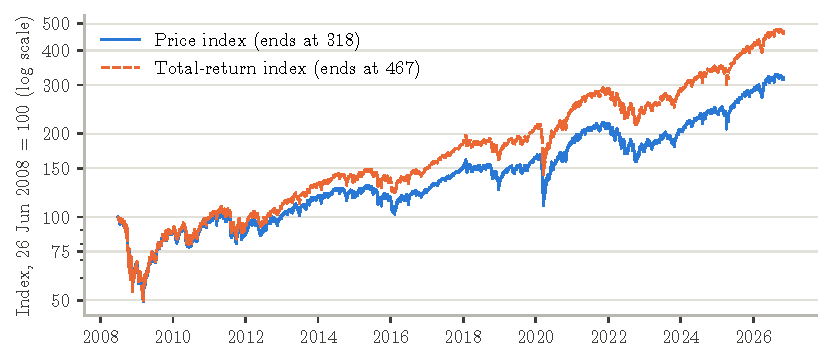
\includegraphics[width=\linewidth]{price.pdf}
\caption{Price index and total-return index (dividends reinvested), both rebased to 100 at inception, log scale. The gap between the two lines is the cumulative contribution of reinvested dividends; equal slopes represent equal percentage returns.}
\end{figure}

\keep{16}\subsection{Calendar-year returns}
\begin{figure}[H]
\centering
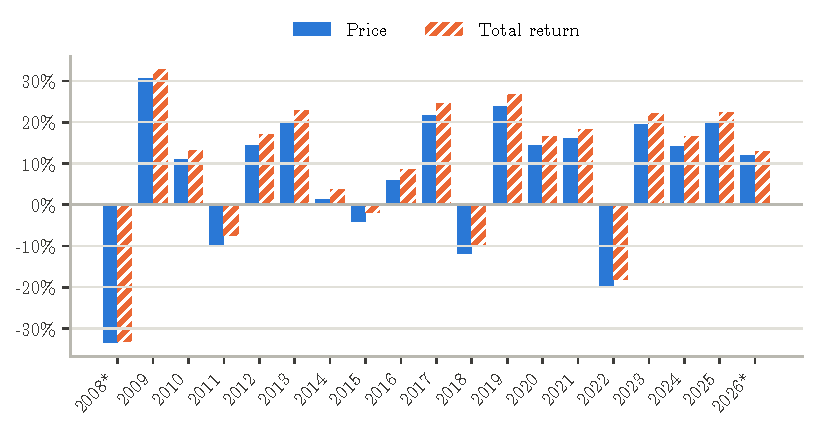
\includegraphics[width=\linewidth]{annual.pdf}
\caption{Calendar-year returns, price and total return. * Partial years.}
\end{figure}
\note{* Partial years: 2008 (from inception) and 2026 (up to 04 Nov 2026). Of the 17 full years, the best was 2009 (+32.7\%) and the worst 2022 ($-$18.0\%); 4 years were negative.}

\keep{16}\subsection{Volatility}
\begin{figure}[H]
\centering
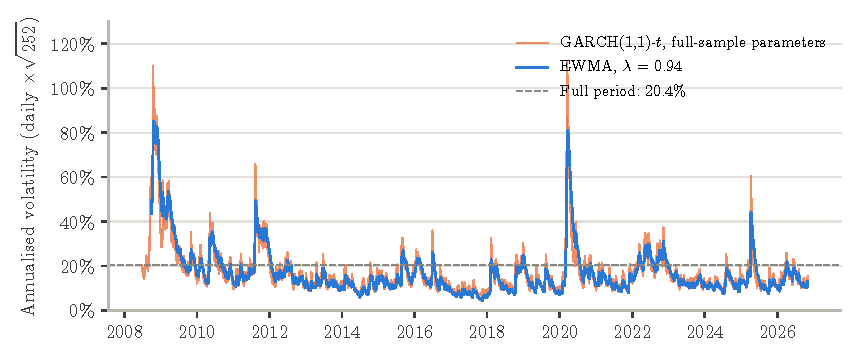
\includegraphics[width=\linewidth]{volatility.pdf}
\caption{Annualised daily volatility: exponentially weighted moving average (RiskMetrics, $\lambda = 0.94$) and GARCH(1,1)-$t$ conditional volatility with parameters estimated on the full sample. Dashed line: full-period volatility on the same daily basis.}
\end{figure}

\begin{table}[H]
\small
\caption{Annualised volatility by sampling frequency (non-overlapping total returns).}
\begin{tabularx}{\linewidth}{L r r}
\toprule
\textbf{Frequency} & \textbf{Observations} & \textbf{Annualised volatility} \\
\midrule
Daily & 4,618 & 20.4\% \\
Weekly & 958 & 18.3\% \\
Monthly & 221 & 16.5\% \\
Quarterly & 74 & 17.8\% \\
\bottomrule
\end{tabularx}
\end{table}
Volatility varies sharply across regimes. The exponentially weighted estimate ranges from 4\% (Nov 2017) to 85\% (23 Oct 2008), and the GARCH conditional volatility peaks at 111\% on 17 Mar 2020. Both measures react within days to a shock and decay as markets calm down. An equally weighted one-year window would instead keep an extreme day at full weight for exactly 252 sessions and then drop it abruptly, creating plateaus that do not reflect the actual level of risk. Both curves use daily returns scaled by $\sqrt{252}$, so the reference line is the full-period figure on the same basis (20.4\%). The GARCH curve uses parameters estimated on the whole sample and is therefore descriptive; the out-of-sample forecasts are evaluated in Section~2.

The annualised level also depends on the sampling frequency. Scaling a $k$-period standard deviation by $\sqrt{k}$ is valid only if returns are serially uncorrelated. Daily returns are negatively autocorrelated (Section~3), so daily data annualised with $\sqrt{252}$ give 20.4\%, whereas monthly data give 16.5\%.

The variance of a sum of $q$ daily returns decomposes into variances and autocovariances:
\[ \operatorname{Var}\Big(\sum_{k=1}^{q} r_k\Big) = q\,\gamma_0\Big[1 + 2\sum_{k=1}^{q-1}\Big(1 - \frac{k}{q}\Big)\rho_k\Big]. \]
With the first 20 daily autocorrelations, the bracket equals 0.71 for $q = 21$: serial dependence alone would reduce the monthly variance to 71\% of 21 times the daily variance. The observed ratio is 0.66, with a 95\% interval of about [0.48, 0.83] from the sampling error of 221 monthly variances (kurtosis of monthly returns 5.1). Autocorrelation thus explains most of the gap, and the remainder is within estimation error. This report uses monthly returns for annualised volatility and for the Sharpe and Sortino ratios.

\keep{16}\subsection{Drawdowns}
\begin{figure}[H]
\centering
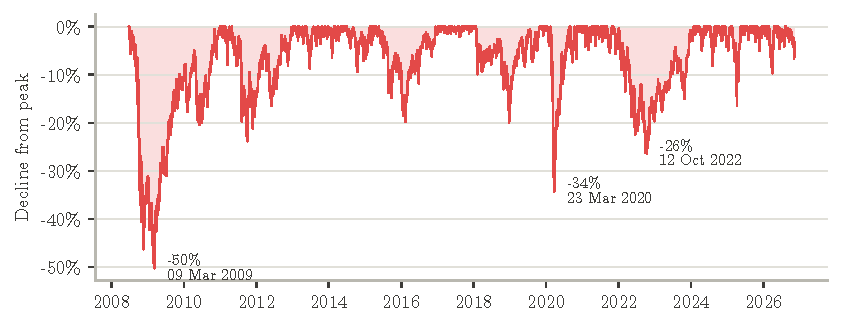
\includegraphics[width=\linewidth]{drawdown.pdf}
\caption{Decline of the total-return index from its previous peak.}
\end{figure}

\begin{table}[H]
\small
\caption{Five largest drawdowns (total return).}
\begin{tabularx}{\linewidth}{l l l R R R}
\toprule
\textbf{Peak} & \textbf{Trough} & \textbf{Recovery} & \textbf{Drawdown} & \textbf{Decline (days)} & \textbf{Recovery (days)} \\
\midrule
26 Jun 2008 & 09 Mar 2009 & 29 Dec 2010 & $-$50.3\% & 175 & 457 \\
12 Feb 2020 & 23 Mar 2020 & 24 Aug 2020 & $-$34.2\% & 27 & 107 \\
08 Nov 2021 & 12 Oct 2022 & 29 Jan 2024 & $-$26.4\% & 233 & 324 \\
29 Apr 2011 & 03 Oct 2011 & 02 Jan 2013 & $-$23.8\% & 108 & 313 \\
26 Jan 2018 & 24 Dec 2018 & 28 Oct 2019 & $-$20.0\% & 229 & 212 \\
\bottomrule
\end{tabularx}
\end{table}
\note{Lengths in trading days. Because VT was launched during the global financial crisis, the first peak is the launch date itself.}

\keep{16}\subsection{Risk-adjusted performance by sub-period}
\begin{table}[H]
\small
\caption{Return and risk by sub-period (total return; volatility and ratios from monthly returns).}
\begin{tabularx}{\linewidth}{L r r r c r r}
\toprule
\textbf{Period} & \textbf{Ann.\ return} & \textbf{Volatility} & \textbf{Sharpe} & \textbf{95\% CI} & \textbf{Sortino} & \textbf{Max.\ DD} \\
\midrule
2008--2012 & 1.9\% & 22.8\% & 0.19 & [$-$0.74, 1.12] & 0.26 & $-$50.3\% \\
2013--2017 & 11.1\% & 10.0\% & 1.07 & [0.15, 1.99] & 1.88 & $-$19.8\% \\
2018--2022 & 5.3\% & 17.9\% & 0.31 & [$-$0.59, 1.20] & 0.44 & $-$34.2\% \\
2023--2026 & 19.2\% & 12.0\% & 1.14 & [0.13, 2.14] & 2.14 & $-$16.5\% \\
\midrule{}Full period & 8.8\% & 16.5\% & 0.51 & [0.03, 0.99] & 0.74 & $-$50.3\% \\
\bottomrule
\end{tabularx}
\end{table}
\note{Excess returns over the 13-week US T-bill (\texttt{\^{}IRX}). Sharpe: mean excess return divided by its volatility. Sortino: mean excess return divided by the downside deviation of excess returns. Confidence intervals for the Sharpe ratio use the standard error of \citet{mertens2002} and \citet{opdyke2007}, which accounts for skewness and kurtosis.}

The confidence intervals are wide: with about five years of monthly data per sub-period, all four sub-period intervals contain the full-period Sharpe ratio, and two contain zero. Differences between sub-periods should be read as descriptive rather than as evidence of a change in the fund's risk-return profile.

% ---------------------------------------------------------------- 2
\keep{24}
\section{Distribution, volatility dynamics and Value at Risk}

\begin{figure}[H]
\centering
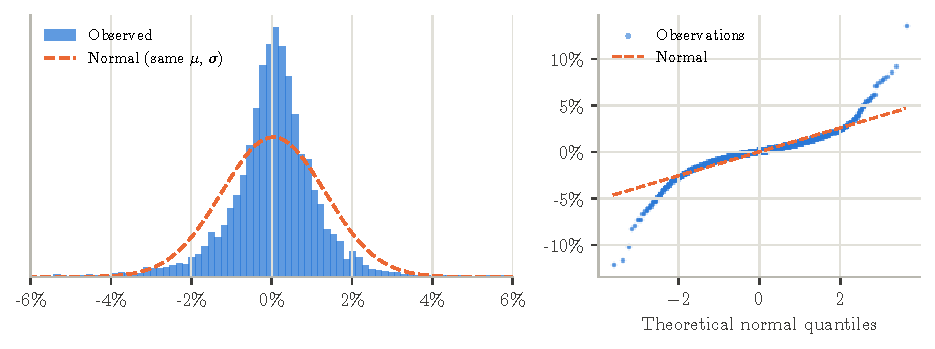
\includegraphics[width=\linewidth]{distribution.pdf}
\caption{Daily total returns: histogram against a normal density with the same mean and variance and a Student-$t$ fitted by maximum likelihood (left), and normal Q--Q plot (right).}
\end{figure}

\begin{table}[H]
\small
\caption{Descriptive statistics of daily returns.}
\begin{tabularx}{\linewidth}{L r r r}
\toprule
\textbf{Statistic} & \textbf{Observed} & \textbf{Normal} & \textbf{Student-$t$} \\
\midrule
Mean / standard deviation & 0.042\% / 1.29\% & same & 0.082\% / 1.55\% \\
Skewness & $-$0.30 & 0 & 0 \\
Kurtosis & 16.08 & 3 & $\infty$ \\
Degrees of freedom $\nu$ & -- & $\infty$ & 2.50 \\
Days beyond $\pm 4$ standard deviations & 47 & 0.29 & 42.7 \\
1\% quantile of daily returns & $-$3.83\% & $-$2.95\% & $-$3.64\% \\
AIC (lower is a better fit) & -- & $-$27,103 & $-$28,828 \\
Jarque--Bera statistic & 33,008 ($p$ $<$ 0.001) & -- & -- \\
Worst day & $-$12.1\% (15 Oct 2008) & -- & -- \\
Best day & +13.5\% (13 Oct 2008) & -- & -- \\
\bottomrule
\end{tabularx}
\end{table}
The tails are far fatter than those of a normal distribution: 47 days moved by more than four standard deviations, whereas a normal distribution would predict 0.3 over the period. The negative skewness means that large declines are more pronounced than large gains. Part of this excess kurtosis reflects time-varying volatility: returns are closer to normal once scaled by their conditional volatility, as the GARCH estimates below show. A Student-$t$ distribution fitted by maximum likelihood has $\nu = 2.5$ degrees of freedom. It reproduces both the sharp peak and the fat tails: its AIC is lower than the normal's by 1,725, and it predicts 42.7 days beyond four standard deviations, against 47 observed. With $\nu < 4$, its theoretical kurtosis is infinite. The GARCH model below finds $\nu = 6.1$ for the shocks scaled by their conditional volatility: much of the unconditional fat-tailedness comes from volatility clustering rather than from the shocks themselves. Being symmetric, the fitted $t$ cannot capture the negative skewness: it still slightly understates the left tail (1\% quantile $-$3.64\% against $-$3.83\% observed).

\keep{16}\subsection{Volatility clustering and GARCH estimates}
\begin{figure}[H]
\centering
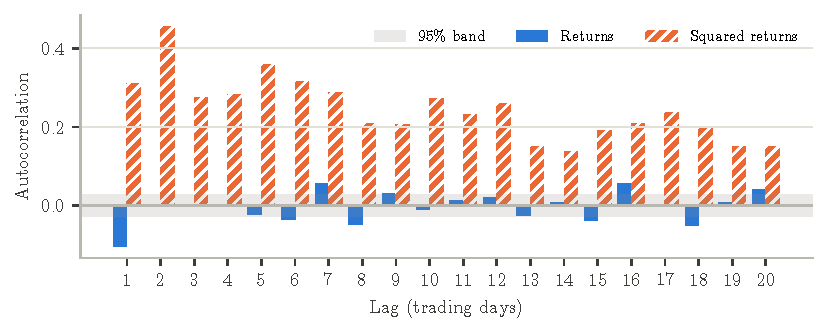
\includegraphics[width=\linewidth]{acf.pdf}
\caption{Autocorrelation of daily log returns and squared log returns, lags 1 to 20, with the 95\% band under independence.}
\end{figure}
Returns show little autocorrelation beyond the first lag (Ljung--Box with 10 lags: $Q = 89.6$). Squared returns, by contrast, are strongly and persistently autocorrelated ($Q = 4,308$, $p < 0.001$): a large move tends to be followed by further large moves of either sign.

\begin{table}[H]
\small
\caption{GARCH(1,1) with standardised Student-$t$ innovations, maximum-likelihood estimates (full sample).}
\begin{tabularx}{\linewidth}{L r r}
\toprule
\textbf{Parameter} & \textbf{Estimate} & \textbf{Standard error} \\
\midrule
$\mu$ (\% per day) & 0.0848 & 0.0110 \\
$\omega$ & 0.0199 & 0.0041 \\
$\alpha$ & 0.1344 & 0.0134 \\
$\beta$ & 0.8584 & 0.0125 \\
$\nu$ (degrees of freedom) & 6.1464 & 0.5496 \\
\bottomrule
\end{tabularx}
\end{table}
\note{Standard errors from the inverse of the numerical Hessian of the log-likelihood.}

The model $\sigma_t^2 = \omega + \alpha\,\varepsilon_{t-1}^2 + \beta\,\sigma_{t-1}^2$ with standardised Student-$t$ innovations is estimated by maximum likelihood on daily log returns in percent \citep{bollerslev1986}. Persistence $\alpha + \beta = 0.993$ implies that a volatility shock loses half its effect after about 97 trading days. The estimated $\nu = 6.1$ confirms that, even after accounting for volatility clustering, daily shocks have fatter tails than the normal distribution. The implied long-run volatility, 26.5\%, uses daily scaling and is therefore comparable with the daily-scaled figure in Section~1.

\keep{16}\subsection{Value at Risk: out-of-sample backtest}
\begin{figure}[H]
\centering
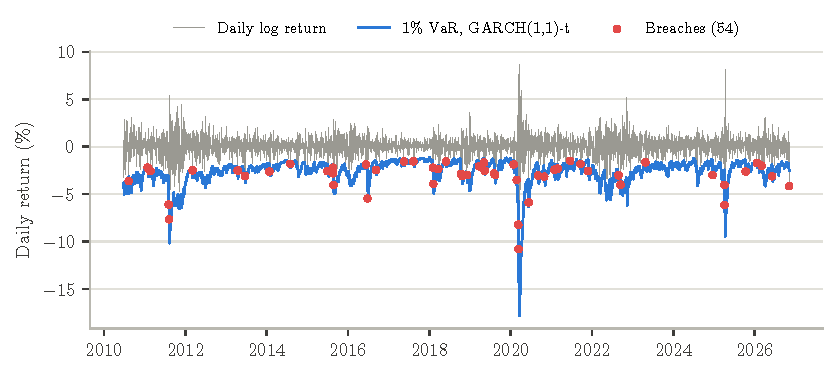
\includegraphics[width=\linewidth]{var_backtest.pdf}
\caption{Daily returns and one-day 1\% VaR forecast by the GARCH(1,1)-$t$ model; red dots mark breaches.}
\end{figure}

\begin{table}[H]
\small
\caption{Backtest of one-day VaR forecasts (4,118 days from 23 Jun 2010); $p$-values of the coverage tests.}
\begin{tabularx}{\linewidth}{l L r r r r r}
\toprule
\textbf{Level} & \textbf{Method} & \textbf{Breach rate} & \textbf{Breaches / expected} & \textbf{Kupiec} & \textbf{Christoff.} & \textbf{CC} \\
\midrule
5\% & Historical (250 days) & 5.20\% & 214 / 206 & 0.565 & $<$ 0.001 & $<$ 0.001 \\
5\% & Normal (250 days) & 5.22\% & 215 / 206 & 0.518 & $<$ 0.001 & $<$ 0.001 \\
5\% & GARCH(1,1)-t & 5.29\% & 218 / 206 & 0.391 & 0.888 & 0.686 \\
1\% & Historical (250 days) & 1.36\% & 56 / 41 & 0.028 & $<$ 0.001 & $<$ 0.001 \\
1\% & Normal (250 days) & 2.38\% & 98 / 41 & $<$ 0.001 & $<$ 0.001 & $<$ 0.001 \\
1\% & GARCH(1,1)-t & 1.29\% & 53 / 41 & 0.076 & 0.005 & 0.004 \\
\bottomrule
\end{tabularx}
\end{table}
\note{One-day VaR on daily log returns, forecasts from 23 Jun 2010 to 04 Nov 2026 (4,118 days), each using only information available the day before. Historical and normal VaR use a 250-day rolling window. GARCH parameters are re-estimated at the start of each calendar year on all prior data, and the conditional variance is updated daily. Kupiec: unconditional coverage; Christoffersen: independence; CC: conditional coverage (joint).}

Rolling historical and normal VaR react slowly to changes in volatility. Their breach rates at 5\% are close to the target, but the breaches cluster in turbulent periods, so the independence test of \citet{christoffersen1998} rejects them decisively. At 1\%, both also fail the unconditional coverage test of \citet{kupiec1995}: 1.36\% and 2.38\% of breaches instead of 1\%. The GARCH(1,1)-$t$ forecasts, from a model estimated with a zero mean, pass both tests at 5\% (breach rate 5.29\%; $p$-values 0.391 and 0.888). At 1\%, their breach rate of 1.29\% is acceptable ($p = 0.076$), but extreme losses still arrive in clusters ($p = 0.005$ for independence). A symmetric $t$ distribution cannot reproduce the negative skewness of large losses; a skewed distribution or an extreme-value model would be the natural next step.

\begin{table}[H]
\small
\caption{GARCH(1,1)-$t$ VaR backtest under three treatments of the conditional mean.}
\begin{tabularx}{\linewidth}{l L r r r r r}
\toprule
\textbf{Level} & \textbf{Mean specification} & \textbf{Breach rate} & \textbf{Breaches / exp.} & \textbf{Kupiec} & \textbf{Christoff.} & \textbf{CC} \\
\midrule
5\% & Zero mean, estimated as such (main) & 5.29\% & 218 / 206 & 0.391 & 0.888 & 0.686 \\
5\% & ML mean kept & 6.07\% & 250 / 206 & 0.002 & 0.824 & 0.009 \\
5\% & ML parameters, mean set to zero afterwards & 5.32\% & 219 / 206 & 0.354 & 0.839 & 0.637 \\
1\% & Zero mean, estimated as such (main) & 1.29\% & 53 / 41 & 0.076 & 0.005 & 0.004 \\
1\% & ML mean kept & 1.48\% & 61 / 41 & 0.004 & 0.014 & $<$ 0.001 \\
1\% & ML parameters, mean set to zero afterwards & 1.26\% & 52 / 41 & 0.103 & 0.004 & 0.004 \\
\bottomrule
\end{tabularx}
\end{table}
The specification of the conditional mean matters. With a symmetric Student-$t$ distribution, the maximum-likelihood location estimate (0.085\% a day) lies well above the sample mean (0.033\%), because negative skewness pulls the mean below the centre of the distribution. Keeping that estimate shifts the VaR upwards and raises the breach rates to 6.07\% and 1.48\%, which the coverage tests reject. The main specification therefore estimates the model with the mean fixed at zero, the usual convention at a one-day horizon. Setting the mean to zero only after estimation gives almost the same breaches, so the conclusion rests on the treatment of the mean, not on how it is imposed.

\keep{16}\subsection{Variance forecasts: out-of-sample comparison}
\begin{table}[H]
\small
\caption{Out-of-sample variance forecasts over the backtest period. Lower losses are better; Diebold--Mariano test of QLIKE against EWMA.}
\begin{tabularx}{\linewidth}{l L r r r r r}
\toprule
\textbf{Horizon} & \textbf{Model} & \textbf{QLIKE} & \textbf{MSE} & \textbf{Rank} & \textbf{DM stat.} & \textbf{$p$-value} \\
\midrule
1 day & Historical variance (250 days) & 1.087 & 20.6 & 3 & 3.87 & $<$ 0.001 \\
1 day & EWMA ($\lambda = 0.94$) & 0.820 & 17.4 & 2 & -- & -- \\
1 day & GARCH(1,1)-$t$ & 0.795 & 16.1 & 1 & $-$2.21 & 0.027 \\
\midrule{}21 days & Historical variance (250 days) & 4.311 & 2,841.0 & 3 & 1.92 & 0.055 \\
21 days & EWMA ($\lambda = 0.94$) & 4.123 & 2,934.1 & 2 & -- & -- \\
21 days & GARCH(1,1)-$t$ & 4.050 & 3,316.3 & 1 & $-$1.47 & 0.141 \\
\bottomrule
\end{tabularx}
\end{table}
\note{Variances in squared percent. Proxy: squared daily return (1 day) and realised variance, the sum of the next 21 squared daily returns (21 days). GARCH: zero-mean model re-estimated each year, multi-step forecasts from its persistence and long-run variance; EWMA and historical variance are held flat over the horizon. Rank by QLIKE. Diebold--Mariano statistics use a Newey--West variance (5 and 25 lags); a negative value favours the model over EWMA.}

A good VaR backtest does not show that a model forecasts variance well, so the three variance forecasts are also compared directly, out of sample, over the same period. QLIKE, $\log h_t + \hat\sigma_t^2/h_t$, and the mean squared error are both robust to noise in the variance proxy \citep{patton2011}; QLIKE penalises under-prediction of risk more heavily and is less dominated by a few extreme days. By QLIKE, GARCH ranks first at both horizons, but the Diebold--Mariano test \citep{diebold1995} against EWMA gives $p = 0.027$ at one day and $p = 0.141$ at 21 days: the improvement over a model with a single fixed parameter is not statistically significant. At one day, EWMA clearly beats the equally weighted 250-day variance ($p$ $<$ 0.001), and GARCH has a lower loss still. By MSE, the ranking changes at 21 days (the 250-day historical variance first), because squared errors are dominated by the few crisis months. The richer model helps describe volatility, but its forecasting advantage is modest.

% ---------------------------------------------------------------- 3
\keep{24}
\section{Market efficiency}

\subsection{First-order autocorrelation}
\begin{table}[H]
\small
\caption{First-order autocorrelation of log returns.}
\begin{tabularx}{\linewidth}{L r r r r r r}
\toprule
\textbf{Frequency} & \textbf{Obs.} & \textbf{$\hat\rho_1$} & \textbf{Naive $t$} & \textbf{Robust $z$} & \textbf{$p$-value} & \textbf{Holm $p$} \\
\midrule
Daily & 4,618 & $-$0.105 & $-$7.16 & $-$2.98 & 0.003 & 0.029 \\
Weekly & 958 & $-$0.023 & $-$0.73 & $-$0.34 & 0.733 & 1.000 \\
Monthly & 221 & 0.033 & 0.49 & 0.32 & 0.745 & 1.000 \\
\bottomrule
\end{tabularx}
\end{table}
\note{Naive $t = \hat\rho_1\sqrt{n}$ assumes independent, identically distributed returns. The robust $z$ uses the heteroskedasticity-consistent standard error $\sqrt{\sum e_t^2 e_{t-1}^2}\,/\sum e_t^2$; $p$-values refer to the robust statistic. Holm: adjusted for the 10 tests of this section.}

Daily autocorrelation is negative ($-$0.105): a gain tends to be slightly reversed the following day. The naive $t$-statistic overstates its significance; the heteroskedasticity-robust statistic is $-$2.98, still significant after the Holm correction. The effect is concentrated in crises: excluding 2008--2009 and February to June 2020, the autocorrelation falls to $-$0.043. Plausible explanations, which these data cannot separate, are overreaction on turbulent days and temporary gaps between the ETF's closing price and the value of its foreign holdings, which trade at different hours. Testing the second would require daily net asset values. At weekly and monthly frequencies, no autocorrelation is detectable.

\keep{16}\subsection{Variance ratio test}
Under the random-walk hypothesis, the variance of $q$-period returns is $q$ times the one-period variance, so
\[
VR(q) = \frac{\operatorname{Var}\left(r_t + r_{t-1} + \dots + r_{t-q+1}\right)}{q \,\operatorname{Var}(r_t)} = 1 .
\]
A ratio below 1 signals mean reversion, a ratio above 1 persistence. Following \citet{lo1988}, the statistic $z^*(q)$ is robust to heteroskedasticity, which is essential given the volatility clustering documented above.

\begin{table}[H]
\small
\caption{Lo--MacKinlay variance ratio test on daily log total returns.}
\begin{tabularx}{\linewidth}{l r r r r R}
\toprule
\textbf{Horizon $q$ (days)} & \textbf{$VR(q)$} & \textbf{$z^*(q)$} & \textbf{$p$-value} & \textbf{Holm $p$} & \textbf{Conclusion (Holm)} \\
\midrule
2 & 0.895 & $-$2.97 & 0.003 & 0.029 & mean reversion \\
5 & 0.830 & $-$2.09 & 0.037 & 0.294 & not rejected \\
10 & 0.777 & $-$1.80 & 0.072 & 0.501 & not rejected \\
20 & 0.759 & $-$1.38 & 0.167 & 1.000 & not rejected \\
\bottomrule
\end{tabularx}
\end{table}

\keep{16}\subsection{Calendar effects}
\begin{figure}[H]
\centering
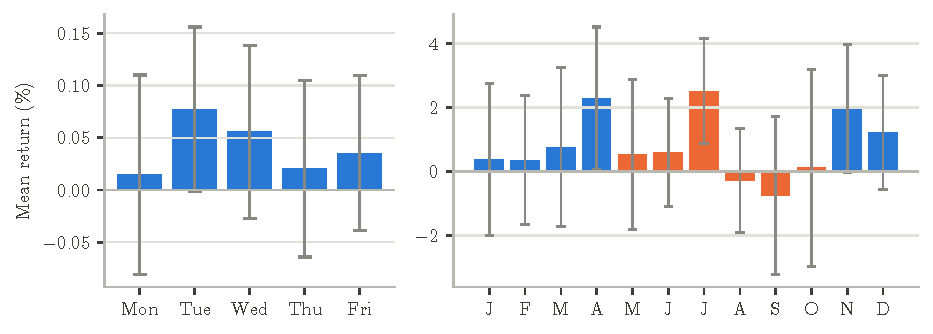
\includegraphics[width=\linewidth]{calendar.pdf}
\caption{Mean daily return by weekday (left) and mean monthly return by calendar month (right), with 95\% confidence intervals. May to October in orange.}
\end{figure}

\begin{table}[H]
\small
\caption{Tests of calendar effects.}
\begin{tabularx}{\linewidth}{L r r r}
\toprule
\textbf{Test} & \textbf{Result} & \textbf{$p$-value} & \textbf{Holm $p$} \\
\midrule
Equal mean returns across weekdays (ANOVA) & $F = 0.38$ & 0.820 & 1.000 \\
January effect: January vs other months (Welch) & 0.38\% vs 0.85\% per month & 0.712 & 1.000 \\
``Sell in May'': Nov--Apr vs May--Oct, per half-year (18 and 18 half-years) & 7.1\% vs 4.7\% & 0.483 & 1.000 \\
\bottomrule
\end{tabularx}
\end{table}
\note{With fewer than twenty observations per calendar month, these tests have little power: the absence of significance does not prove the absence of an effect, only that any effect is too small to detect in eighteen years of data.}

\keep{12}\subsection{Multiple testing}
Section~3 reports 10 hypothesis tests. If all null hypotheses were true and the tests independent, 0.5 false rejections would be expected at the 5\% level, and the probability of at least one would be about 40\%. Each $p$-value is also adjusted with the step-down procedure of \citet{holm1979}, which controls the probability of any false rejection. 3 tests are significant before adjustment and 2 after. Both remaining rejections concern the same first-order daily autocorrelation, since $VR(2) \approx 1 + \hat\rho_1$.

\keep{16}\subsection{Moving-average timing rules}
\begin{figure}[H]
\centering
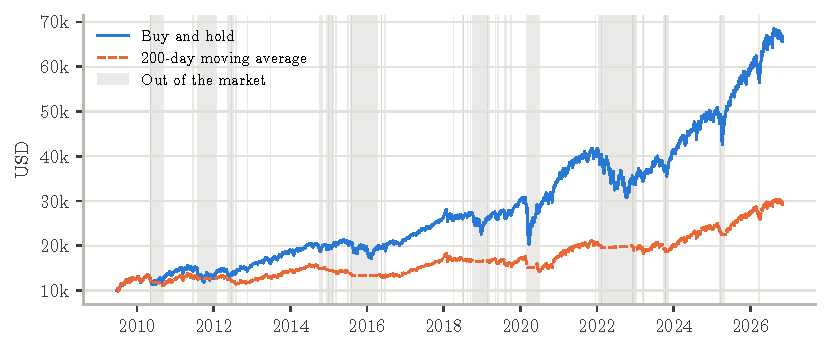
\includegraphics[width=\linewidth]{ma200.pdf}
\caption{Growth of USD 10{,}000 from 24 Jun 2009: buy and hold vs the 200-day moving-average rule. Shaded areas: rule out of the market.}
\end{figure}

\begin{table}[H]
\small
\caption{Buy and hold vs 200-day moving average (Sharpe ratio with 95\% confidence interval).}
\begin{tabularx}{\linewidth}{L r r}
\toprule
 & \textbf{Buy and hold} & \textbf{200-day moving average} \\
\midrule
Annualised return & 11.5\% & 6.5\% \\
Volatility & 14.7\% & 11.2\% \\
Sharpe ratio & 0.72 [0.22, 1.21] & 0.49 [0.01, 0.96] \\
Maximum drawdown & $-$34.2\% & $-$22.5\% \\
Final value of USD 10{,}000 & USD 66,709 & USD 29,697 \\
\bottomrule
\end{tabularx}
\end{table}

\begin{table}[H]
\small
\caption{Sensitivity to the moving-average window and to execution (common period). Volatility, Sharpe and drawdown refer to the main execution.}
\begin{tabularx}{\linewidth}{L r r r r r r r}
\toprule
\textbf{Window} & \textbf{Ann.\ return} & \textbf{Delayed} & \textbf{Volatility} & \textbf{Sharpe} & \textbf{Max.\ DD} & \textbf{Switches} & \textbf{Invested} \\
\midrule
50 days & 3.6\% & 4.2\% & 9.6\% & 0.26 & $-$25.9\% & 319 & 68\% \\
100 days & 5.9\% & 5.3\% & 10.3\% & 0.47 & $-$25.2\% & 203 & 72\% \\
150 days & 5.6\% & 7.5\% & 10.7\% & 0.42 & $-$26.9\% & 177 & 74\% \\
200 days & 6.5\% & 7.1\% & 11.2\% & 0.49 & $-$22.5\% & 140 & 77\% \\
250 days & 6.4\% & 6.4\% & 11.0\% & 0.48 & $-$23.1\% & 141 & 77\% \\
\midrule{}Buy and hold & 11.5\% & 11.5\% & 14.7\% & 0.72 & $-$34.2\% & 0 & 100\% \\
\bottomrule
\end{tabularx}
\end{table}
\note{Rule: the position earning the return of day $t$ is decided with prices up to the close of day $t-1$, so no future information is used. The main case assumes the trade is executed at that same close (a market-on-close order placed just before the close); the delayed case executes one session later. Out of the market, the rule earns the T-bill rate; each switch costs 0.10\%. All windows are compared over the same period, starting 24 Jun 2009, the first day on which a 250-day average is available.}

Every window underperformed buy and hold, by 5.1\% to 8.0\% a year, while reducing the maximum drawdown. For the 200-day rule, a circular block bootstrap (2,000 replications, 63-day blocks) gives a 95\% confidence interval of [0.0\%, 10.2\%] for the annual return gap ($p = 0.050$): the underperformance is borderline significant. The sample starts in mid-2009, after the financial-crisis crash that such rules are designed to avoid, which works against them; a longer index history would be needed for a fair assessment. Late and repeated signals (``whipsaws'') are costly in a market that recovers quickly. Delaying execution by one session changes the results by up to 1.9\% a year, in both directions: the ranking of windows is fragile, but the underperformance against buy and hold is not.

% ---------------------------------------------------------------- 4
\keep{24}
\section{Holding period and investor behaviour}

\subsection{Rolling returns and the probability of loss}
\begin{figure}[H]
\centering
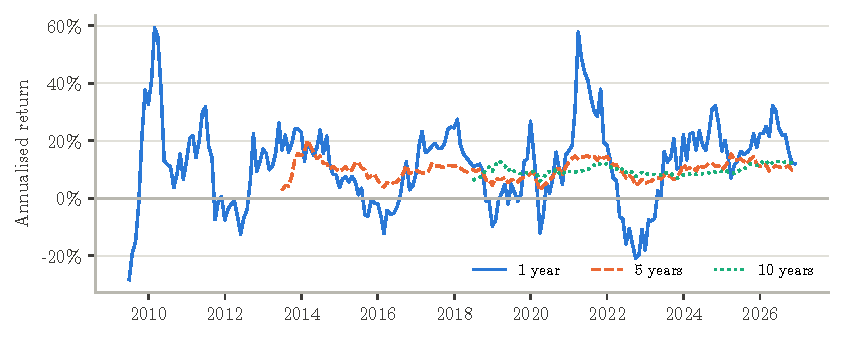
\includegraphics[width=\linewidth]{rolling.pdf}
\caption{Annualised total return over rolling 1-, 5- and 10-year windows, by end of window.}
\end{figure}

\begin{table}[H]
\small
\caption{Rolling returns (overlapping monthly windows, annualised) and bootstrap probability of loss.}
\begin{tabularx}{\linewidth}{l r r r R r r}
\toprule
\textbf{Horizon} & \textbf{Windows} & \textbf{P(loss)} & \textbf{Bootstrap} & \textbf{Worst (window end)} & \textbf{Median} & \textbf{Best} \\
\midrule
1 year & 210 & 22\% & 24\% & $-$28.4\% (Jun 2009) & 13.1\% & 59.3\% \\
5 years & 162 & 0\% & 10\% & 2.8\% (Mar 2020) & 10.1\% & 20.0\% \\
10 years & 102 & 0\% & 4\% & 6.0\% (Mar 2020) & 9.3\% & 13.1\% \\
\bottomrule
\end{tabularx}
\end{table}
Overlapping windows understate the probability of loss at long horizons: the 10-year windows contain only about one and a half independent periods, none of which happened to lose money. A stationary bootstrap \citep{politis1994} that resamples blocks of monthly returns (mean length 12 months, 20,000 paths) gives a more defensible estimate: 10\% over five years and 4\% over ten.

These figures are fragile. The Monte Carlo error is negligible (about 0.1 percentage point), but the estimate depends on the assumed block length, which governs how much of the slow-moving dependence in returns is preserved: from 1\% to 6\% over ten years across the block lengths tested. Above all, no resampling scheme can capture the uncertainty about the true expected return. Treating monthly log returns as independent and normal, the probability of a ten-year loss is 6\%; moving the mean return to either end of its 95\% confidence interval gives 0.1\% to 45\%. Eighteen years of data simply do not pin down the long-run probability of loss.

\begin{table}[H]
\footnotesize
\begin{minipage}[t]{0.48\linewidth}
\caption{Bootstrap probability of loss by mean block length (months).}
\begin{tabularx}{\linewidth}{L r r r}
\toprule
\textbf{Block} & \textbf{1 year} & \textbf{5 years} & \textbf{10 years} \\
\midrule
1 (i.i.d.) & 30\% & 13\% & 5.6\% \\
6 & 24\% & 13\% & 6.0\% \\
12 (main) & 25\% & 10\% & 4.0\% \\
24 & 24\% & 7\% & 1.9\% \\
36 & 24\% & 5\% & 1.0\% \\
\bottomrule
\end{tabularx}
\end{minipage}\hfill
\begin{minipage}[t]{0.48\linewidth}
\caption{Normal i.i.d. model: probability of loss with the mean at its estimate and at the ends of its 95\% interval.}
\begin{tabularx}{\linewidth}{L r r r}
\toprule
\textbf{Horizon} & \textbf{Estimate} & \textbf{High $\mu$} & \textbf{Low $\mu$} \\
\midrule
1 year & 31\% & 16.9\% & 48\% \\
5 years & 13\% & 1.6\% & 46\% \\
10 years & 6\% & 0.1\% & 45\% \\
\bottomrule
\end{tabularx}
\end{minipage}
\end{table}

\keep{16}\subsection{Sensitivity to the starting date}
\begin{figure}[H]
\centering
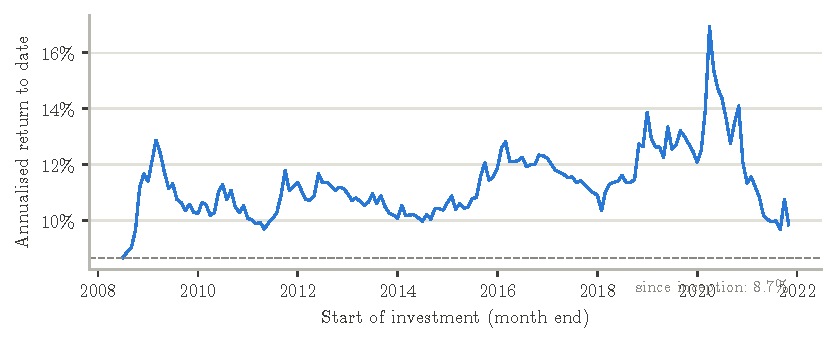
\includegraphics[width=\linewidth]{start_date.pdf}
\caption{Annualised total return from each month end to the latest close (starting points with at least five years of history).}
\end{figure}
Because VT was launched just before the 2008 crash, ``since inception'' figures are among the least favourable available. Starting at any year end between 2008 and 2021 would have delivered between 10.2\% (2010) and 14.1\% (2018) a year to date, against 8.8\% since inception. Performance statistics should always be read together with their start and end dates.

\keep{16}\subsection{The cost of missing the best days}
\begin{figure}[H]
\centering
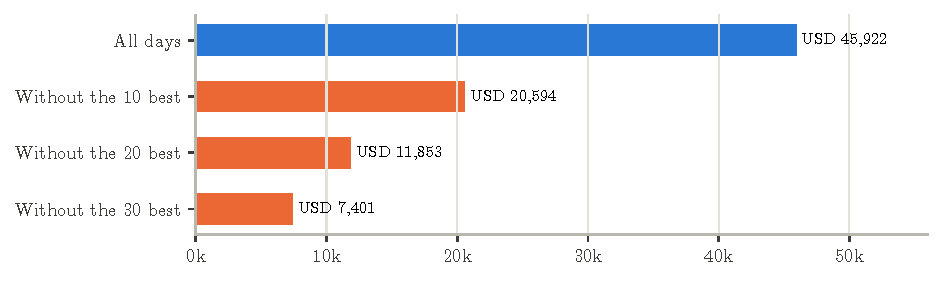
\includegraphics[width=\linewidth]{best_days.pdf}
\caption{Final value of USD 10{,}000 invested at inception, with and without the best trading days.}
\end{figure}
Missing the 10 best days out of 4,618 cuts the annualised return from 8.8\% to 4.1\%. The reverse exercise is just as striking: avoiding the 10 worst days would have lifted the final value to USD 114,330. 7 of the 10 best days fall within two weeks of one of the 10 worst. They occur in the same crisis periods: avoiding the worst days without missing the best would require perfect timing.

\keep{16}\subsection{Monthly savings plan and lump-sum investing}
\begin{figure}[H]
\centering
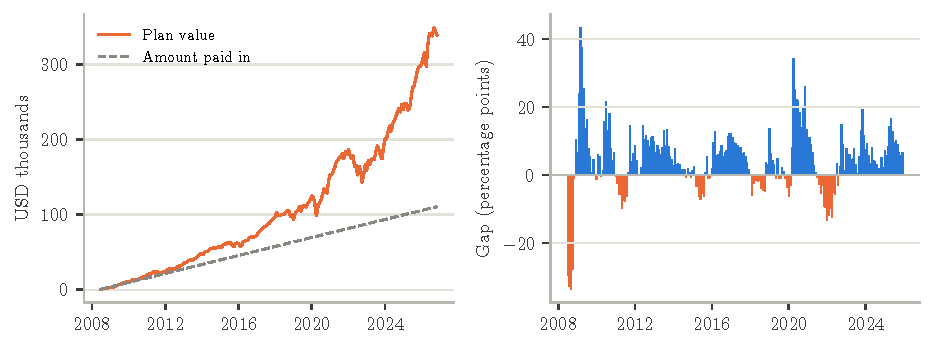
\includegraphics[width=\linewidth]{savings.pdf}
\caption{Left: value of a USD 500 monthly plan vs amount paid in. Right: lump sum minus 12-month averaging, value gap after 12 months, by starting month.}
\end{figure}
Investing USD 500 at the end of every month since inception (221 contributions, USD 110,500 in total) would be worth USD 344,656 today, an internal rate of return of 11.3\% a year, above the 8.8\% of a single investment at inception because most of the money was invested after the 2008--2009 crash.

Across the 210 possible monthly starting points, investing a sum all at once beat spreading it over 12 months (with the uninvested cash earning the T-bill rate) in 72\% of cases, with an average advantage of 4.6\% after 12 months. Because the market rises most of the time, waiting costs money on average; averaging in mainly limits the regret of investing just before a decline. The starting points overlap, so this frequency is descriptive rather than a precise probability.

% ---------------------------------------------------------------- 4.5 Kelly
\keep{20}\subsection{Optimal leverage, Kelly criterion and volatility drag}
\label{sec:kelly}
Can leverage raise the long-run compounded growth of an investment in VT, and by how much? This subsection derives the growth-optimal exposure, estimates it, tests it out of sample and separates the effects that make leveraged compounding differ from a simple multiple of the fund's return. The aim is not to show that leverage pays, but to identify the assumptions under which it maximises expected growth and to show how fragile that optimum is.

\paragraph{Framework.} Suppose the fund's value follows a geometric Brownian motion with arithmetic expected return $\mu$ and volatility $\sigma$, and an investor holds a constant exposure $L$ to it, rebalanced continuously, with the rest in cash at the rate $r_f$ ($L<1$) or financed by borrowing ($L>1$). $L=1$ is the unleveraged fund, $L=0.5$ a 50\% exposure and $L=2$ a 200\% exposure. If borrowing costs $r_f$, wealth $W$ grows at the expected logarithmic rate
\[
g(L) = \frac{1}{\mathrm{d}t}\,\mathbb{E}\left[\mathrm{d}\log W_t\right] = r_f + L(\mu - r_f) - \tfrac{1}{2}L^2\sigma^2 .
\]
The arithmetic expected return of the portfolio, $r_f + L(\mu - r_f)$, rises linearly with $L$, but the expected log growth carries the quadratic penalty $\tfrac{1}{2}L^2\sigma^2$. Since $g'(L) = (\mu - r_f) - L\sigma^2$ and $g''(L) = -\sigma^2 < 0$, the function is strictly concave and maximised at the Kelly exposure \citep{kelly1956,breiman1961,merton1969}
\[
L^* = \frac{\mu - r_f}{\sigma^2}, \qquad g(L^*) = r_f + \frac{(\mu - r_f)^2}{2\sigma^2}.
\]
$\mu$ is an arithmetic mean: substituting the historical CAGR, which is already a log-growth rate net of the drag $\tfrac12\sigma^2$, would count the drag twice.

\paragraph{Borrowing costs.} A retail investor borrows above the rate earned on cash. With a lending rate $r_l$ and a borrowing rate $r_b > r_l$, the growth rate is piecewise:
\[
g(L) = \begin{cases} r_l + L(\mu - r_l) - \tfrac12 L^2\sigma^2, & 0 \le L \le 1,\\[2pt] r_b + L(\mu - r_b) - \tfrac12 L^2\sigma^2, & L > 1. \end{cases}
\]
It remains concave, with a kink at $L=1$. The optimum is $(\mu - r_l)/\sigma^2$ if that is below one, $(\mu - r_b)/\sigma^2$ if that is above one, and exactly one otherwise: leverage is worth taking only if the marginal expected return exceeds the marginal borrowing cost by more than the marginal variance penalty. Margin rates are not available in the data, so the borrowing rate is set to the T-bill yield plus a spread of 1.5\% a year, comparable to the lower end of retail margin rates; Table~\ref{tab:ksens} reports spreads from 0 to 3\%. The T-bill yield itself is a lending rate, not an observable margin rate.

\paragraph{Simulation.} The strategies are simulated on daily simple total returns $r_t$ from the adjusted prices, so dividends are included and fund expenses, already in the price, are not charged again. For an exposure $L$ decided at the close of day $t-1$,
\[
W_t = W_{t-1}\left(1 + R_{p,t} - c_t\right), \qquad R_{p,t} = \begin{cases} L r_t + (1-L)\, r_{l,t}, & 0\le L\le1,\\ L r_t - (L-1)\, r_{b,t}, & L>1, \end{cases}
\]
where $r_{l,t}$ is the T-bill yield known at the previous close divided by 252, $r_{b,t} = r_{l,t} + \text{spread}/252$, and $c_t$ is a cost of 2\,bp per unit of exposure traded when the position is rebalanced to its target at the close. With $L=1$ nothing is traded and the simulation reproduces buy-and-hold exactly. If $1 + R_{p,t} - c_t \le 0$, the strategy is insolvent and its wealth stays at zero. Five numerical checks are run on every update: $L=1$ reproduces the fund's total-return path, $L=0$ reproduces the cash account, the closed-form $L^*$ matches the numerical maximum of $g$, the exact decomposition below reconciles with simulated wealth to machine precision, and wealth cannot recover after insolvency.

\begin{table}[H]
\small
\caption{Kelly inputs and leverage estimates (full sample).}
\label{tab:kelly}
\begin{tabularx}{\linewidth}{L r}
\toprule
\textbf{Input} & \textbf{Estimate} \\
\midrule
Arithmetic mean return $\mu$ (daily mean $\times 252$) & 10.5\% \\
Cash rate $r_f$ (13-week T-bill, average) & 1.4\% \\
Expected excess return $\mu - r_f$ (standard error) & 9.1\% (4.8\%) \\
Volatility $\sigma$, daily returns $\times\sqrt{252}$ & 20.4\% \\
Volatility $\sigma$, monthly returns $\times\sqrt{12}$ & 16.5\% \\
Borrowing rate (assumption) & T-bill $+$ 1.5\% \\
\midrule
\textbf{Exposure} & \\
Theoretical Kelly, borrowing at the T-bill rate, daily variance (In-sample, hindsight) & 2.19x \\
Theoretical Kelly, borrowing at the T-bill rate, monthly variance (In-sample, hindsight) & 3.07x \\
Theoretical Kelly, borrowing spread 1.5\% (In-sample, hindsight) & 1.83x \\
Ex-post log-growth maximiser, frictionless (Exact daily recursion) & 2.14x \\
Ex-post log-growth maximiser, spread and 2\,bp costs (Exact daily recursion) & 1.78x \\
Half Kelly / quarter Kelly (from the spread case) (Fractional) & 0.91x / 0.46x \\
Feasible under Regulation T initial margin (Constraint) & $\le$ 2.00x \\
\bottomrule
\end{tabularx}
\end{table}
With daily rebalancing, the variance that governs compounding is the variance of daily returns. Using it, the frictionless Kelly exposure is 2.19x; with the assumed borrowing spread it falls to 1.83x. The exact daily recursion, which needs neither the diffusion approximation nor normality, is maximised at 2.14x without frictions and at 1.78x with the spread and rebalancing costs, close to the theoretical values. The monthly variance gives 3.07x: because daily returns are negatively autocorrelated (Section~3), the Kelly exposure depends on the rebalancing frequency it is meant for. All these figures are computed on the full sample and are therefore in-sample and hindsight-calibrated: they describe what would have maximised growth over this particular history, not an achievable ex-ante optimum.

\begin{figure}[H]
\centering
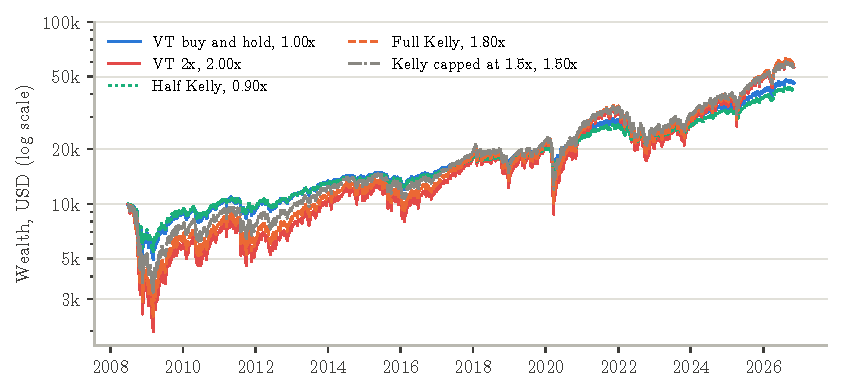
\includegraphics[width=\linewidth]{kelly_wealth.pdf}
\caption{Historical simulation, not a forecast: growth of USD 10{,}000 under constant exposures rebalanced daily, borrowing at the T-bill rate plus 1.5\%, 2\,bp rebalancing costs. Kelly exposures are estimated on the full sample (hindsight).}
\end{figure}

\begin{table}[H]
\small
\caption{Constant-exposure strategies, full sample, daily rebalancing, borrowing spread 1.5\%. Volatility and Sharpe ratio from monthly returns, as in Section~1.}
\label{tab:kstrat}
\begin{tabularx}{\linewidth}{L r r r r r r r}
\toprule
\textbf{Strategy} & \textbf{$L$} & \textbf{CAGR} & \textbf{Vol.} & \textbf{Sharpe} & \textbf{Max.\ DD} & \textbf{Final (USD)} & \textbf{Margin days} \\
\midrule
VT buy and hold & 1.00x & 8.8\% & 16.5\% & 0.51 & $-$50.3\% & 46,707 & 0 \\
VT 2x & 2.00x & 10.1\% & 33.3\% & 0.42 & $-$80.1\% & 58,201 & 0 \\
Quarter Kelly & 0.46x & 5.2\% & 7.5\% & 0.53 & $-$25.3\% & 25,493 & 0 \\
Half Kelly & 0.91x & 8.3\% & 15.0\% & 0.51 & $-$46.7\% & 43,028 & 0 \\
Full Kelly & 1.83x & 10.2\% & 30.4\% & 0.43 & $-$76.3\% & 59,343 & 0 \\
Kelly capped at 1.5x & 1.50x & 10.0\% & 24.9\% & 0.45 & $-$67.7\% & 57,623 & 0 \\
VT 3x & 3.00x & 6.6\% & 50.2\% & 0.37 & $-$93.6\% & 32,082 & 2 \\
VT 4x & 4.00x & $-$1.6\% & 66.9\% & 0.34 & $-$98.4\% & 7,490 & 2140 \\
\bottomrule
\end{tabularx}
\end{table}
Leverage raised the historical CAGR only up to a point. Full Kelly (1.83x) and 2x ended with about 59k and 58k against 47k for buy and hold, a gain of roughly 1.4\% a year, bought with maximum drawdowns of $-$76\% and $-$80\% instead of $-$50\%. Their Sharpe ratios are lower than buy and hold, not higher: leverage financed above the cash rate scales risk more than excess return. At 3x, the CAGR drops to 6.6\%, and at 4x to $-$1.6\% with a $-$98\% drawdown: beyond the optimum, more leverage lowers long-run growth. Quarter and half Kelly give up most of the growth gain but cut drawdowns sharply, the usual argument for fractional Kelly. The four objectives that appear in this table, log growth, Sharpe ratio, maximum drawdown and terminal wealth in one realised path, are different and point to different exposures.

The simulation is frictionless in one important respect: it assumes the target exposure can always be restored at the close. In practice, a US margin account is limited by Regulation T to an initial loan of 50\% of the purchase price (2x), and FINRA Rule 4210 requires equity of at least 25\% of the position's value, with many brokers demanding more. The last column counts the days on which equity fell below 25\% of assets before rebalancing, a proxy for a margin call. A 3x position, which starts with 33\% equity, breaches the threshold on 2 days (15 Oct 2008, 16 Mar 2020), when VT fell by more than 11\% in a single session; a 4x position starts at the 25\% limit and breaches it on almost every down day. A forced sale at such moments would lock in the loss and break the constant-leverage path assumed here.

\paragraph{Volatility drag and the compounding gap.} Three different effects separate a leveraged position from ``$L$ times the fund'', in addition to trading costs. To isolate the effect of leverage on compounding, compare the frictionless daily-reset position financed at a rate $b_t$ with the geometrically scaled reference $\log W^{\text{ref}}_T = L\sum_t \log(1+r_t) - (L-1)\sum_t\log(1+b_t)$. The difference is
\begin{align*}
D_T(L) &= \sum_{t=1}^{T}\Big[\log\big(1 + L r_t - (L-1) b_t\big) - L\log(1+r_t) + (L-1)\log(1+b_t)\Big] \\
&\approx -\tfrac12 L(L-1)\sum_{t=1}^{T}(r_t - b_t)^2 ,
\end{align*}
where the approximation uses second-order expansions of the logarithms and requires every wealth factor to be positive \citep{cheng2009,avellaneda2010}. The gap is zero for $L=0$ and $L=1$, negative for $L>1$, and grows with realised variance and with $L(L-1)$.

\begin{table}[H]
\small
\caption{Exact decomposition of annualised log growth, full sample, spread 1.5\%, 2\,bp costs. Components add up to the total.}
\label{tab:kdecomp}
\setlength{\tabcolsep}{4pt}
\begin{tabularx}{\linewidth}{l R R R R R R}
\toprule
\textbf{$L$} & \textbf{$L\times$ log growth of VT} & \textbf{T-bill financing} & \textbf{Borrowing spread} & \textbf{Compoun\-ding gap} & \textbf{Trading costs} & \textbf{Total log growth} \\
\midrule
1.00x & 8.4\% & 0.0\% & 0.0\% & 0.0\% & 0.00\% & 8.4\% \\
1.50x & 12.6\% & $-$0.7\% & $-$0.7\% & $-$1.6\% & $-$0.03\% & 9.5\% \\
2.00x & 16.8\% & $-$1.4\% & $-$1.5\% & $-$4.2\% & $-$0.08\% & 9.6\% \\
3.00x & 25.2\% & $-$2.8\% & $-$3.0\% & $-$12.8\% & $-$0.25\% & 6.4\% \\
\bottomrule
\end{tabularx}
\end{table}
Over the full sample, VT's arithmetic mean return was 10.5\% a year, but its log growth only 8.4\%: the difference, 2.1\%, is the ordinary volatility drag that affects any risky investment, close to $\tfrac{1}{2}\sigma^2 = 2.1\%$. Leverage adds a second, distinct effect. Table~\ref{tab:kdecomp} decomposes the realised log growth of each strategy exactly into five parts: $L$ times the log growth of VT; financing at the T-bill rate; the borrowing spread; the compounding gap $D_T(L)$; and trading costs. At 2x, the compounding gap costs 4.2\% a year, more than the T-bill financing (1.4\%) or the spread (1.5\%), and costs are negligible. At 3x the gap grows to 12.8\%, roughly in proportion to $L(L-1)$ as the approximation predicts.

\begin{figure}[H]
\centering
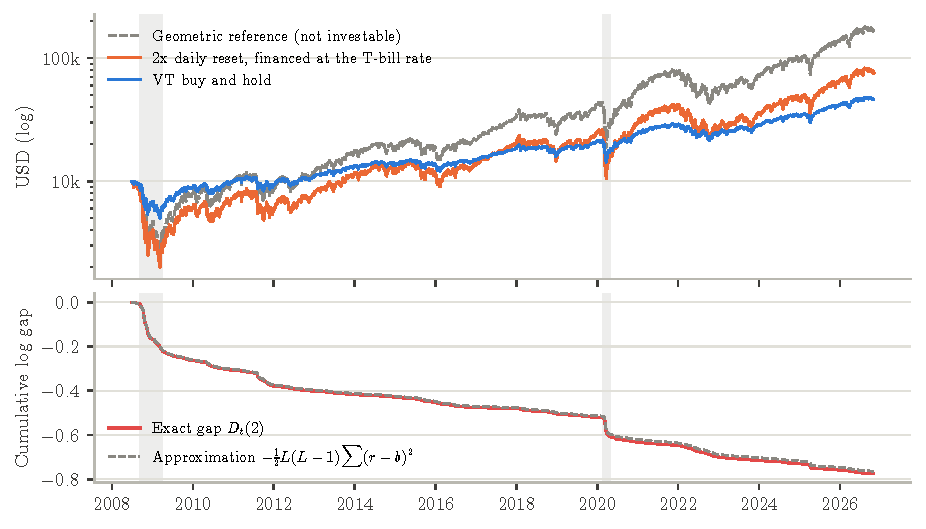
\includegraphics[width=\linewidth]{kelly_drag.pdf}
\caption{Historical simulation: a frictionless 2x daily-reset position financed at the T-bill rate, its geometrically scaled reference and VT (top); cumulative exact compounding gap and its approximation (bottom). Shaded: September 2008 to March 2009 and February to April 2020.}
\end{figure}
The gap is path-dependent. If VT gains 10\% and then loses 9.09\%, it is back where it started; a daily-reset 2x position gains 20\% and then loses 18.18\%, ending 1.8\% lower ($1.2 \times 0.8182 = 0.982$). Over the sample, the exact gap at 2x reached -0.775 in log terms (approximation -0.764), so the frictionless 2x position ended at USD 77,795 against USD 168,927 for the geometric reference. Most of the gap accumulated in the 2008--2009 and 2020 crises, when daily variance was highest. The reference is a decomposition device, not an investable strategy. Compared with another common benchmark, twice the cumulative simple return of VT (USD 83,413), the daily-reset position also ended lower in this sample, but that comparison has no fixed sign: in a steady trend with low volatility, daily resetting compounds gains and can beat the simple multiple.

\paragraph{Growth as a function of leverage.} Figure~\ref{fig:kgrowth} plots the model growth curve and the growth actually realised by each constant exposure. The curves are concave: below the optimum, more leverage adds growth; beyond it, the quadratic penalty dominates and growth falls, turning negative around 4x. The realised curve follows the model closely because both use the same sample, which is precisely why its maximum is not a guide to the future. The shaded band shows how far the model curve moves when $\mu$ is set to either end of its 95\% confidence interval: the uncertainty grows with $L$, and at 2x the band is 37 percentage points of annual growth wide.

\begin{figure}[H]
\centering
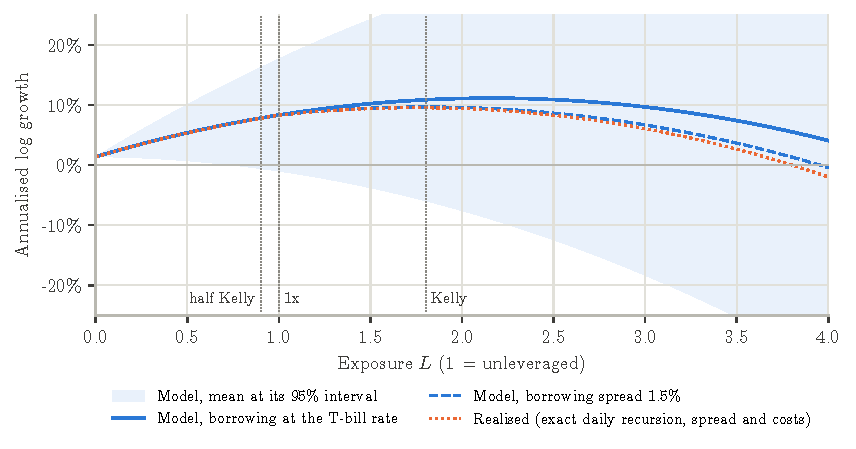
\includegraphics[width=\linewidth]{kelly_growth.pdf}
\caption{Model-implied expected log growth $g(L)$ (blue, with and without the borrowing spread; band: mean return at the ends of its 95\% interval) and realised log growth of the daily simulations (orange, in-sample). Vertical lines: 1x, half Kelly and Kelly with the spread.}
\label{fig:kgrowth}
\end{figure}

\paragraph{Estimation uncertainty.} Kelly leverage inherits the imprecision of the expected return. With $\hat\mu - r_f = 9.1\%$ estimated with a standard error of 4.8\%, the approximate standard error of $L^*$ is $1/(\sigma\sqrt{T}) \approx 1.14$. The block bootstrap confirms it: with 21-day blocks, the 95\% interval runs from 0.25x to 4.78x, the probability that the true optimum is below 1x is 12\%, and the results hardly depend on the block length. Table~\ref{tab:ksens} shows that plausible changes to the expected return, the variance or the period move the estimate by about one unit of leverage or more: an excess return of 3\% instead of the historical 9.1\% gives 0.72x; the GARCH long-run variance gives 1.30x; and the five-year sub-periods range from 0.69x to 7.10x.

\begin{table}[H]
\small
\caption{Circular block bootstrap of the frictionless Kelly exposure (2,000 resamples of daily excess returns).}
\begin{tabularx}{\linewidth}{L r r r r}
\toprule
\textbf{Block length} & \textbf{Median} & \textbf{95\% interval} & \textbf{P($L^*<1$)} & \textbf{P($L^*>2$)} \\
\midrule
1 (i.i.d.) & 2.23x & [$-$0.11x, 4.43x] & 15\% & 59\% \\
21 days & 2.24x & [0.25x, 4.78x] & 12\% & 57\% \\
63 days & 2.25x & [0.21x, 4.98x] & 13\% & 59\% \\
252 days & 2.20x & [0.31x, 5.44x] & 13\% & 57\% \\
\bottomrule
\end{tabularx}
\end{table}

\begin{table}[H]
\small
\caption{Kelly exposure under alternative inputs, one input changed at a time (borrowing at the T-bill rate unless stated).}
\label{tab:ksens}
\begin{tabularx}{\linewidth}{l L r}
\toprule
\textbf{Input} & \textbf{Value} & \textbf{$L^*$} \\
\midrule
Expected excess return & Historical estimate & 2.19x \\
Expected excess return & Excess return 5\% & 1.20x \\
Expected excess return & Excess return 3\% & 0.72x \\
\midrule{}Variance estimate & Daily returns, $\sigma = 20.4\%$ & 2.19x \\
Variance estimate & Monthly returns, $\sigma = 16.5\%$ & 3.34x \\
Variance estimate & GARCH long run, $\sigma = 26.5\%$ & 1.30x \\
\midrule{}Borrowing spread & 0.0\% & 2.19x \\
Borrowing spread & 0.5\% & 2.07x \\
Borrowing spread & 1.5\% & 1.83x \\
Borrowing spread & 3.0\% & 1.47x \\
\midrule{}Sub-period & 2008--2012 & 0.69x \\
Sub-period & 2013--2017 & 6.99x \\
Sub-period & 2018--2022 & 1.42x \\
Sub-period & 2023--2026 & 7.10x \\
\bottomrule
\end{tabularx}
\end{table}

\paragraph{Out-of-sample test.} To remove hindsight, Kelly exposure is re-estimated at every month end from 30 Jun 2011, after a 3-year training period, using only data available at that date: the expanding-window mean excess return, the expanding-window daily variance and the current T-bill yield plus the spread. The estimate is held for the next month and rebalanced daily. It ranged from 0.03x to 1.86x, starting at 0.64x because the training period was dominated by the 2008 crash; caps at 1.5x or 2x would never have bound. Out of sample, estimated full Kelly earned 9.8\% a year against 10.2\% for buy and hold, with higher volatility and a lower Sharpe ratio; the leverage that looks optimal in hindsight was not identifiable in real time. Fixed 2x did better over this particular period, which began after the crash, but choosing it also relies on hindsight.

\begin{figure}[H]
\centering
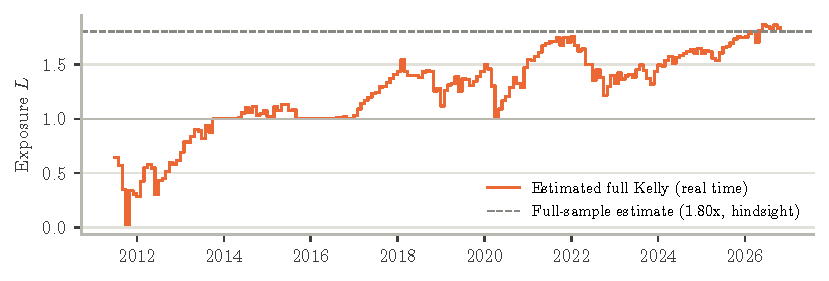
\includegraphics[width=\linewidth]{kelly_oos.pdf}
\caption{Kelly exposure estimated in real time at each month end (expanding window, borrowing spread 1.5\%), compared with the full-sample estimate available only in hindsight.}
\end{figure}

\begin{table}[H]
\small
\caption{Out-of-sample comparison from 01 Jul 2011 (common period, daily rebalancing, spread 1.5\%, 2\,bp costs).}
\label{tab:koos}
\begin{tabularx}{\linewidth}{L r r r r r r}
\toprule
\textbf{Strategy} & \textbf{$L$: mean (range)} & \textbf{CAGR} & \textbf{Vol.} & \textbf{Sharpe} & \textbf{Max.\ DD} & \textbf{Final (USD)} \\
\midrule
VT buy and hold & 1.00x & 10.2\% & 14.3\% & 0.64 & $-$34.2\% & 44,306 \\
VT 2x & 2.00x & 14.2\% & 29.0\% & 0.55 & $-$59.6\% & 76,282 \\
Full-sample Kelly, 1.83x (hindsight) & 1.83x & 13.7\% & 26.5\% & 0.56 & $-$55.8\% & 71,800 \\
Estimated full Kelly (real time) & 1.25x (0.03x--1.86x) & 9.8\% & 18.1\% & 0.52 & $-$44.0\% & 41,833 \\
Estimated half Kelly (real time) & 0.63x (0.01x--0.93x) & 6.5\% & 9.0\% & 0.57 & $-$24.0\% & 26,206 \\
\bottomrule
\end{tabularx}
\end{table}

\paragraph{Interpretation.} Historical VT returns imply a growth-optimal exposure of about 1.83x with realistic borrowing costs, but this number is an in-sample artefact of one favourable eighteen-year path rather than a parameter that can be relied on. Its 95\% interval spans almost the whole range from no leverage to 4x, it moves by about one unit of leverage or more with plausible changes to the expected return, the variance or the period, and a real-time estimate would not have found it. The features documented earlier in this report work against aggressive leverage: fat tails and volatility clustering (Section~2) mean that losses arrive in bursts, exactly when the compounding gap widens and margin calls occur; the 50\% drawdown of 2008--2009 becomes 76\% at full Kelly and 80\% at 2x; and the confidence interval of the Sharpe ratio (Section~1) is the same uncertainty that makes $L^*$ unknowable. Because the growth curve is flat near its maximum and falls steeply beyond it, overestimating $L^*$ is far more costly than underestimating it. This asymmetry is the case for fractional Kelly \citep{thorp2006,maclean2011}: under the model, half Kelly keeps three quarters of the growth gain while halving the volatility, and at the point estimate it does not even require borrowing.

% ---------------------------------------------------------------- 5
\keep{24}
\section{A Swiss investor's perspective}
\begin{figure}[H]
\centering
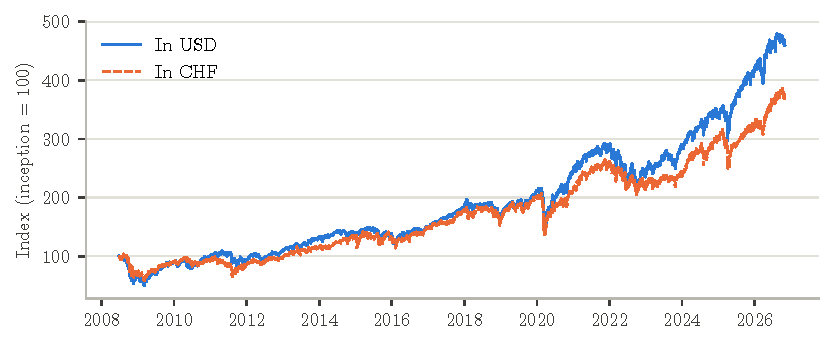
\includegraphics[width=\linewidth]{chf.pdf}
\caption{Total return in USD and in CHF, rebased to 100 at inception.}
\end{figure}

\begin{table}[H]
\small
\caption{VT in US dollars and in Swiss francs.}
\begin{tabularx}{\linewidth}{L r r}
\toprule
 & \textbf{In USD} & \textbf{In CHF} \\
\midrule
Annualised total return & 8.8\% & 7.4\% \\
Annualised volatility (monthly returns) & 16.5\% & 14.9\% \\
USD/CHF over the period & -- & 1.0237 $\rightarrow$ 0.8166 ($-$1.2\% a year) \\
Correlation of VT with USD/CHF (weekly / daily) & -- & $-$0.24 / $-$0.05 \\
Risk-free rate (average) & T-bill, 1.4\% & SARON, $-$0.1\% \\
Sharpe ratio, 95\% confidence interval & 0.51 [0.03, 0.99] & 0.56 [0.07, 1.05] \\
\bottomrule
\end{tabularx}
\end{table}
The dollar depreciated against the franc, costing an unhedged Swiss investor about 1.3\% of return a year. The weekly correlation between VT and USD/CHF is $-$0.24; the daily correlation, $-$0.05, is biased towards zero because Yahoo's daily currency and ETF closes are taken at different times of day. The dollar tends to strengthen against the franc when equities fall, which cushions part of the losses in CHF. Because VT is a global fund, its true exposure is to a basket of currencies: USD/CHF captures only part of the currency effect. All figures are before Swiss income tax and the 15\% US withholding tax on dividends, which a Swiss resident can usually credit against Swiss tax. Measured against the investor's own risk-free rate, SARON for the franc and the T-bill for the dollar, the Sharpe ratio is 0.56 in CHF against 0.51 in USD. The franc risk-free rate averaged $-$0.1\% over the period, against 1.4\% for the T-bill.

\begin{table}[H]
\small
\caption{Downside risk in US dollars and in Swiss francs (total return).}
\begin{tabularx}{\linewidth}{L r r}
\toprule
 & \textbf{In USD} & \textbf{In CHF} \\
\midrule
One-day 5\% VaR, GARCH(1,1)-t: breaches / expected (Kupiec $p$) & 218 / 206 (0.391) & 200 / 206 (0.672) \\
One-day 1\% VaR, GARCH(1,1)-t: breaches / expected (Kupiec $p$) & 53 / 41 (0.076) & 56 / 41 (0.028) \\
Probability of loss over 1 / 5 / 10 years: historical windows & 22\% / 0\% / 0\% & 23\% / 0\% / 0\% \\
Probability of loss over 1 / 5 / 10 years: block bootstrap & 24\% / 10\% / 4\% & 25\% / 10\% / 4\% \\
\bottomrule
\end{tabularx}
\end{table}
The VaR backtest and the probability of loss are repeated on the total return in CHF, with the same methods. At the 1\% level, the GARCH(1,1)-t forecast has 56 breaches in CHF against 53 in USD (about 41 expected); the Kupiec test rejects correct coverage in CHF but not in USD. Part of the difference may come from Yahoo's USD/CHF and VT closes being taken at different times of day, which adds noise to daily CHF returns; the model is otherwise estimated exactly as in USD. Over one to ten years, the bootstrap probability of loss differs by at most 0.3 percentage point between the two currencies: the weaker dollar lowered the CHF return, but CHF returns were also less volatile.

% ---------------------------------------------------------------- 6
\keep{24}
\section{Data validation}
\begin{table}[H]
\small
\caption{Total returns from Yahoo adjusted prices vs Vanguard's published returns, to 30 September 2026.}
\begin{tabularx}{\linewidth}{L r r r r}
\toprule
\textbf{Period} & \textbf{Vanguard, market price} & \textbf{This report} & \textbf{Gap (pp)} & \textbf{Vanguard, NAV} \\
\midrule
Third quarter 2026 & 0.83\% & 0.83\% & +0.00 & 0.76\% \\
Year to date & 12.86\% & 12.86\% & $-$0.00 & 12.83\% \\
1 year & 16.45\% & 16.45\% & +0.00 & 16.32\% \\
3 years & 21.46\% & 21.45\% & $-$0.01 & 21.42\% \\
5 years & 11.36\% & 11.35\% & $-$0.01 & 11.34\% \\
10 years & 12.32\% & 12.32\% & $-$0.00 & 12.32\% \\
Since inception & 8.78\% & 8.81\% & +0.03 & 8.78\% \\
\bottomrule
\end{tabularx}
\end{table}
\note{Periods of one year or more are annualised. Source: Vanguard fact sheet F3141 (data as of 30 September 2026), stored in \texttt{data/reference/}.}

Yahoo's adjusted prices are not an official source, so the total returns used in this report were checked against the market-price returns published by Vanguard. For all standard periods the two agree to within 0.01 percentage point. The small gap since inception arises because Vanguard measures from the launch on 24 June 2008, two trading days before the first Yahoo closing price. The ETF's market price and its net asset value (NAV) also track each other closely.

% ---------------------------------------------------------------- 7
\keep{20}
\section{Limitations}
\begin{itemize}[leftmargin=1.2em,itemsep=0.3em,topsep=0.2em]
  \item \textbf{One asset, one period.} All results come from a single fund over eighteen years that include one global financial crisis, one pandemic crash and a long bull market. Estimates of mean returns and Sharpe ratios are imprecise over such horizons, as the confidence intervals show.
  \item \textbf{Start date.} VT was launched just before the 2008 crash, which depresses every ``since inception'' figure and works against timing rules that would have protected investors during that crash.
  \item \textbf{Data source.} Yahoo Finance is not an official source, and its adjusted prices can be revised retroactively. The validation against Vanguard covers a single reference date.
  \item \textbf{Market price vs NAV.} The analysis uses closing market prices. The daily autocorrelation may partly reflect gaps between the market price and the net asset value, which cannot be tested without daily NAV data.
  \item \textbf{Taxes and costs.} Returns are gross of investor-level taxes and trading costs (fund expenses are already reflected in the price). Dividends are assumed to be reinvested at the closing price on the ex-dividend date.
  \item \textbf{Leverage simulations.} Section~\ref{sec:kelly} assumes the target exposure is restored at each close at a small cost, ignores intraday moves, forced liquidations and taxes, and uses an assumed borrowing spread rather than observed margin rates. Its results are historical simulations, not achievable track records.
  \item \textbf{Model choices.} GARCH(1,1) with symmetric Student-$t$ errors does not capture the asymmetric response of volatility to losses (leverage effect) nor the skewness of large losses. Bootstrap results assume that the dependence structure of the past repeats.
\end{itemize}

% ---------------------------------------------------------------- 8
\keep{12}
\section{Conclusion}
The evidence describes a broadly diversified equity fund that has delivered the equity risk premium with the usual features of equity returns: fat tails, volatility that clusters and persists, and deep but temporary drawdowns.

Three statements about efficiency need to be kept apart. Statistically, the random walk is rejected only for a small negative daily autocorrelation; failing to reject it at longer horizons does not prove that prices are efficient, because the tests have limited power with eighteen years of data. In terms of predictability, the effect explains about 1.1\% of the variance of daily returns and is concentrated in crises. Economically, none of the simple rules examined, moving averages or calendar strategies, created value after costs. The data are consistent with an efficient market at the horizons that matter to investors, without proving it.

Leverage illustrates the same point from another angle. Over this sample, a Kelly exposure of about 1.83x would have maximised growth after borrowing costs, but the estimate is too imprecise to act on, a real-time version did not beat buy and hold, and the compounding gap, deep drawdowns and margin constraints all bite hardest in the crises that dominate long-run outcomes.

On risk, the richer models help to describe volatility, but their forecasting advantage over a simple exponentially weighted average is modest, and every model still underestimates how extreme losses cluster. For long-term investors, the lessons are about horizon and discipline rather than prediction: the probability of loss falls with the holding period but remains uncertain and not negligible, and missing a handful of days in the middle of a crisis is as costly as suffering the worst of it.

\section*{Data, methods and reproducibility}
\note{Source: Yahoo Finance, downloaded with the \texttt{yfinance} library and updated automatically (GitHub repository \url{https://github.com/cedricmasset98/vt}). VT: daily closing prices and prices adjusted for dividends and splits (``Adj Close''). Risk-free rate: 13-week US T-bill (\texttt{\^{}IRX}); in CHF, SARON monthly average from the Swiss National Bank data portal (cube \texttt{zimoma}). Currency: USD/CHF (\texttt{CHF=X}). Annualised returns use calendar time; annualised volatility, Sharpe and Sortino ratios use monthly returns; Sharpe confidence intervals follow \citet{mertens2002} and \citet{opdyke2007}, allowing for skewness and kurtosis. Bootstrap results use the fixed seed 20080626. Data file fingerprint (SHA-256 of \texttt{data/VT.csv}): \texttt{8d4044535e242353}. Software: Python 3.13.17, pandas 3.0.5, NumPy 2.5.3, SciPy 1.18.1, Matplotlib 3.11.2. The five numerical checks of Section~\ref{sec:kelly} passed on this run (largest error 1.6e-14); they are also run as \texttt{tests/test\_kelly.py} before each update. These analyses are descriptive and historical; they do not constitute investment advice.}

\begin{thebibliography}{99}
\footnotesize
\setlength{\itemsep}{0.2em}
\bibitem[Avellaneda and Zhang(2010)]{avellaneda2010}
Avellaneda, M. and Zhang, S. (2010). Path-dependence of leveraged ETF returns. \emph{SIAM Journal on Financial Mathematics}, 1(1), 586--603.
\bibitem[Bollerslev(1986)]{bollerslev1986}
Bollerslev, T. (1986). Generalized autoregressive conditional heteroskedasticity. \emph{Journal of Econometrics}, 31(3), 307--327.
\bibitem[Breiman(1961)]{breiman1961}
Breiman, L. (1961). Optimal gambling systems for favorable games. In \emph{Proceedings of the Fourth Berkeley Symposium on Mathematical Statistics and Probability}, Vol.~1, 65--78. University of California Press.
\bibitem[Cheng and Madhavan(2009)]{cheng2009}
Cheng, M. and Madhavan, A. (2009). The dynamics of leveraged and inverse exchange-traded funds. \emph{Journal of Investment Management}, 7(4), 43--62.
\bibitem[Christoffersen(1998)]{christoffersen1998}
Christoffersen, P.~F. (1998). Evaluating interval forecasts. \emph{International Economic Review}, 39(4), 841--862.
\bibitem[Diebold and Mariano(1995)]{diebold1995}
Diebold, F.~X. and Mariano, R.~S. (1995). Comparing predictive accuracy. \emph{Journal of Business \& Economic Statistics}, 13(3), 253--263.
\bibitem[Holm(1979)]{holm1979}
Holm, S. (1979). A simple sequentially rejective multiple test procedure. \emph{Scandinavian Journal of Statistics}, 6(2), 65--70.
\bibitem[Kelly(1956)]{kelly1956}
Kelly, J.~L. (1956). A new interpretation of information rate. \emph{Bell System Technical Journal}, 35(4), 917--926.
\bibitem[Kupiec(1995)]{kupiec1995}
Kupiec, P.~H. (1995). Techniques for verifying the accuracy of risk measurement models. \emph{Journal of Derivatives}, 3(2), 73--84.
\bibitem[Lo and MacKinlay(1988)]{lo1988}
Lo, A.~W. and MacKinlay, A.~C. (1988). Stock market prices do not follow random walks: Evidence from a simple specification test. \emph{Review of Financial Studies}, 1(1), 41--66.
\bibitem[MacLean, Thorp and Ziemba(2011)]{maclean2011}
MacLean, L.~C., Thorp, E.~O. and Ziemba, W.~T. (Eds.) (2011). \emph{The Kelly Capital Growth Investment Criterion: Theory and Practice}. World Scientific.
\bibitem[Merton(1969)]{merton1969}
Merton, R.~C. (1969). Lifetime portfolio selection under uncertainty: The continuous-time case. \emph{Review of Economics and Statistics}, 51(3), 247--257.
\bibitem[Mertens(2002)]{mertens2002}
Mertens, E. (2002). Comments on variance of the IID estimator in Lo (2002). Working paper, University of Basel.
\bibitem[Opdyke(2007)]{opdyke2007}
Opdyke, J.~D. (2007). Comparing Sharpe ratios: So where are the p-values? \emph{Journal of Asset Management}, 8(5), 308--336.
\bibitem[Patton(2011)]{patton2011}
Patton, A.~J. (2011). Volatility forecast comparison using imperfect volatility proxies. \emph{Journal of Econometrics}, 160(1), 246--256.
\bibitem[Politis and Romano(1994)]{politis1994}
Politis, D.~N. and Romano, J.~P. (1994). The stationary bootstrap. \emph{Journal of the American Statistical Association}, 89(428), 1303--1313.
\bibitem[Thorp(2006)]{thorp2006}
Thorp, E.~O. (2006). The Kelly criterion in blackjack, sports betting, and the stock market. In S.~A. Zenios and W.~T. Ziemba (Eds.), \emph{Handbook of Asset and Liability Management}, Vol.~1, 385--428. Elsevier.
\end{thebibliography}

\end{document}